~\vspace{.1in}

\section{Logistic and other growth models}

A flu virus has been spreading through the college dormitories. Initially 8 students were diagnosed with the flu, but that number has been growing rapidly.  After 2 weeks, there were 64 students with the flu.   We are interested in predicting how many students will catch the flu over the next 6 weeks or so.  To get a sense of scale, there are \text{1,094} students currently living in the dorms. 

The variables are
\begin{center}
\begin{tabular} {l} 
$D=$ time since first cases (days) $\sim$ indep \\
$F= $ total number of students with the flu (students) $\sim$ dep \\ 
\end{tabular}
\end{center}

One model estimates that the number of students diagnosed with the flu was growing 16\% per day.  (If this story sounds familiar, it's because the story also appears in the practice exercises 2.2 \#3 and 5.1 \#2.)  The corresponding equation is
$$\textbf{exponential:} \quad F = 8 \ast 1.16^D$$
As a check, at 14 days there were
$$F = 8 \ast 1.16^{14} = 8 \times 1.16 \wedge \underline{14} = 63.900143\ldots \approx 64 \text{ students}$$
We rounded the numbers in our table to the nearest person. 

\begin{center}
\begin{tabular} {|c| |c|c|c |c|c |c|c|}\hline
$D$ & 0 & 7 & 14 & 21 & 28 & 35 & 42 \\ \hline
$F$ (\textbf{exponential}) & 8 & 23 & 64 & 181 & 510 & \text{1,442} & \text{4,077} \\ \hline
\end{tabular}
\end{center}

While at first the exponential model seems reasonable, it quickly gets too large to make sense.  After all, there are only  \text{1,094} students currently living in the dorms so the numbers we found at 5 and 6 weeks (also known as 35 and 42 days) are totally unrealistic.   The exponential model is based on the assumption that the rate of change of the number of new cases is proportional to the number of \textbf{infected} students: those who already have the flu.  

There are both advantages and disadvantages of the exponential model.  To it's credit, the exponential model captures the reality of the first few weeks, where the flu spreads very rapidly.  But, the exponential model misses several basic facts.  First, as more students catch the flu, the number of new cases decreases in part because sick people are already surrounded by sick people so there aren't new people to get sick.  Second, for whatever reasons, not everyone is going to catch the flu no matter how exposed they are.  We would like to have an alternative model that keeps what works (rapid increase at first) but deals better with the long term (the growth slows down and not everyone catches the flu).  There are two different models we consider that have these properties:  saturation and logistic.

The first example is a \textbf{saturation} model.  Basically it assumes that the rate of change of the number of new cases is proportional to the number of \textbf{susceptible} students: those who are likely to catch the flu but haven't already.  Since at the beginning many susceptible students don't have the flu, it spreads very quickly, even faster than the exponential does.  But once most susceptible students have caught the flu, the number of new cases dwindles.  

Leaving out the details of how we found it, a possible saturation equation for our example is
$$\textbf{saturation:} \quad F=96-88\ast.93^D$$  
As a check, initially there were
$$F = 96-88 \ast .93^0 = 96 - 88 \times .93 \wedge \underline{0} = 8 \text{ students} \quad \checkmark$$
and at 14 days there were
$$F = 96-88 \ast .93^{14} = 96 - 88 \times .93 \wedge \underline{14} =64.1401334\ldots \approx 64 \quad \checkmark$$
We rounded the numbers in our table to the nearest person. 
\begin{center}
\begin{tabular} {|c| |c|c|c  |c|c| c|c|}\hline
$D$ & 0 & 7 & 14 & 21 & 28 & 35 & 42 \\ \hline
$F$ (\textbf{saturation}) & 8 & 43 & 64 & 77 & 85 & 89 &92 \\ \hline
\end{tabular}
\end{center}
The saturation model predicts that 92 students (total) will have (or have had) the flu over the next 6 weeks.

The second example is a \textbf{logistic} (or \textbf{S-curve}) model.  Basically it assumes that the rate of change of the number of new cases is jointly proportional to the number of infected students and the number of susceptible students.  It acknowledges the heavy influence the number of infected students have initially on the growth, but balances it with the limiting influence of the diminishing number of susceptible students over time.

It turns out that a possible logistic equation for our example is
$$\textbf{logistic:} \quad F=\frac{129}{1+15 \ast .825^D}$$  
For example, initially there were
$$F = \frac{129}{1+15\ast .825^0} = 129 \div ( 1 + 15 \times .825 \wedge \underline{0}) = 
8.0625000\ldots \approx 8 \text{ students} \quad \checkmark$$
and at 14 days there were
$$F = \frac{129}{1+15\ast .825^{14}} = 129 \div ( 1 + 15 \times .825 \wedge \underline{14}) = 64.0212993\ldots \approx 64 \text{ students} \quad \checkmark$$
Notice how we need parentheses around the bottom of our fraction, as usual, to override the normal order of operations.  We rounded the numbers in the table to the nearest person. 
\begin{center}
\begin{tabular} {|c| |c|c|c |c|c| c|c|}\hline
$D$ & 0 & 7 & 14 & 21 & 28 & 35 & 42  \\ \hline
$F$ (\textbf{logistic}) & 8 & 26 & 64 & 102 & 121 & 127 & 128\\ \hline
\end{tabular}
\end{center}
The logistic model projects that 128 students (total) will have (or have had) the flu over the next 6 weeks, considerably more than projected by the saturation model.

Here are all three models on the same graph.
\begin{center}
\scalebox {1} {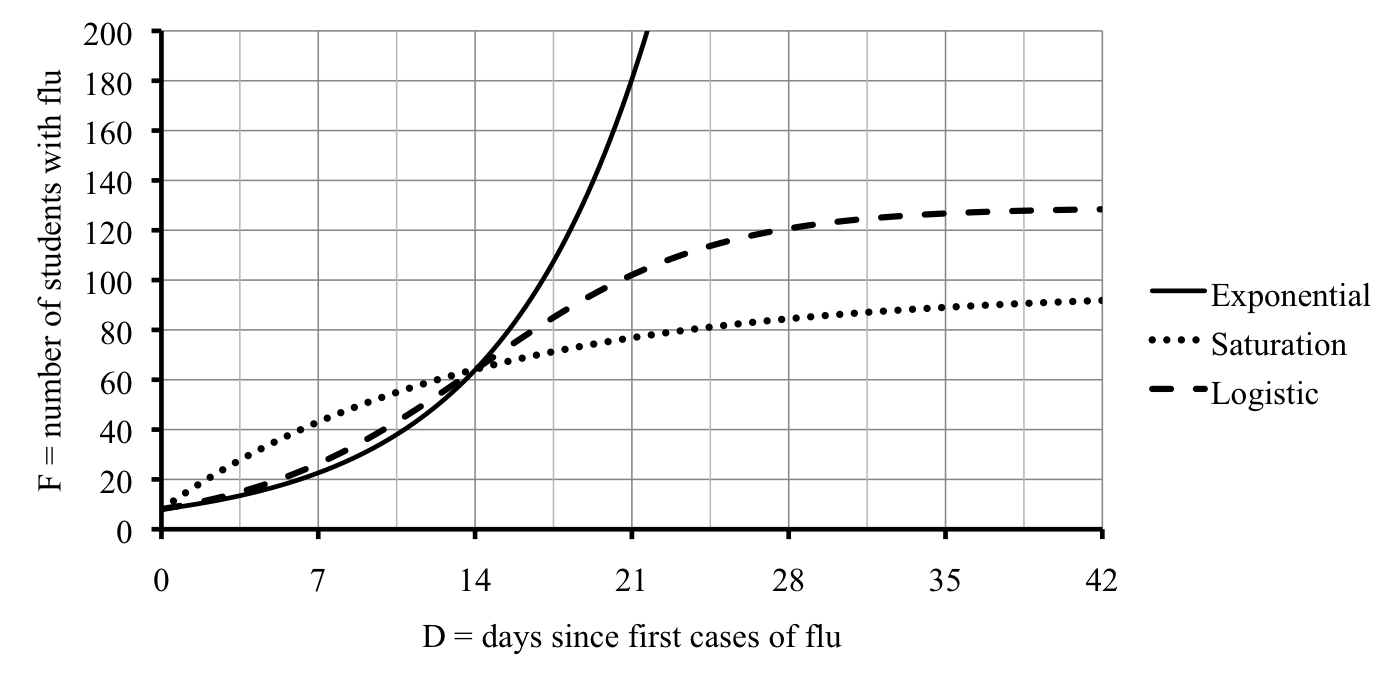
\includegraphics [width = 6in] {flumodels.png}}
\end{center}
As you can see from the graph, both the saturation and logistic curves level off as expected.  One way to estimate those \textbf{limiting values} (or \textbf{carrying capacity}) is to evaluate the functions at large values, say 60 days, 100 days, and (the unrealistic) \text{1,000} days.

\vspace{.05in} %VSPACE
\begin{center}
\begin{tabular} {|c| |c |c |c|}\hline
$D$ & 60 & 100 & \text{1,000}\\ \hline
$F$ (\textbf{exponential})  & $\cancel{\approx \text{59,000}}$ & $\cancel{\approx \text{22 million}}$ & $\cancel{\approx 1.35 \times 10^{33}}$\\ \hline
$F$ (\textbf{saturation})  & 94.86 & 95.94 & 96.00\\ \hline
$F$ (\textbf{logistic}) & 128.98 & 128.99 & 129.00\\ \hline
\end{tabular}
\end{center}
\vspace{.05in} %VSPACE

We crossed out the unrealistic values from the exponential equation.  So, if the saturation model is accurate, then we should expect around 96 total cases.  But, if the logistic model is accurate, then we should expect around 129 total cases instead.

Look back at the equations:
\vspace{.05in} %VSPACE
\begin{center}
\begin{tabular} {ll} 
 \textbf{saturation:} & $F=96-88\ast.93^D$ \\ 
 \begin{tiny} ~ \end{tiny} \\
 \textbf{logistic:} & $\displaystyle F=\frac{129}{1+15 \ast .825^D}$ \\
\end{tabular}
\end{center} 
\vspace{.05in} %VSPACE
The limiting values were there all along!

%\section{Logistic and other growth models}  

 \begin{center}
\line(1,0){300} %\line(1,0){250}
\end{center}

\section*{Homework}

\noindent \textbf{Start by doing Practice exercises \#1-4 in the workbook.}

\bigskip

\noindent \textbf{Do you know \ldots}  

\begin{itemize}
\item Why we might use a logistic or saturation model, instead of an exponential model?
\item The difference between a logistic and saturation model?

\item What the limiting value of a logistic function means in the story and what it tells us about the graph? 
\item How to find the limiting value of a logistic function?  
\item What the graph of a logistic function looks like? 

\item What the limiting value of a saturation function means in the story and what it tells us about the graph? 
\item How to find the limiting value of a saturation function?  
\item What the graph of a saturation function looks like? 

\item[~] \textbf{If you're not sure, work the rest of exercises and then return to these questions.  Or, ask your instructor or a classmate for help.}  
\end{itemize}

\subsection*{Exercises}

%Narrative = lily pads on a pond?  STart with french school girls story with exponential, then try saturation model, then logistic.  Follow structure of Bolker

\begin{enumerate} 
\setcounter{enumi}{4}
\item In our example in this section, we made several tables of values.  Go back and check that they are correct.

\item Mari volunteers answering calls for in the office of her local state government representative.  The office has been receiving a lot of calls recently with about BPA, a chemical found in plastics.  The callers want their representative to support a bill banning BPA.  An equation that describes the number of total number of calls over time is the following:
$$ C=\frac{837}{1+118\ast 0.8025^D}$$ % Logistic  NOTE:  cumulative count
where $D$ is the time since January 1 (in days), and $C$ is the total number of calls.

\begin{enumerate}
\item According to this equation, how many calls (total) will Mari's office get by February 1 (day 31), March 1 (day 59), April 1 (day 90), May 1 (day 120), and Nov 8 (day 311)?
\item During which months did most of the calls come in? 
\item Draw a graph illustrating the function.
\item Describe what happened over time.
\end{enumerate}

\item Even though all the callers support the bill, Mari isn't sure whether the calls represent the local constituents.  Perhaps only supporters are calling her office, for example.  So, she asks her pollster, Paul, to add this question to the list for his daily survey.  Based on that survey, Paul estimates the percentage $P$ of local constituents who support the bill on day $D$ by the equation $$P =100 - 87.3 \ast 0.992^D$$ %Saturating 
\begin{enumerate}
\item According to this equation, what percentage of callers supported the bill on January 1 (day 0), March 1 (day 59), Aug 1 (day 212), Oct 1 (day 273) and Nov 8 (day 311)?
\item What does your equation say the percentage would be on day 500 (which probably isn't realistic in this problem)?  How about day 1,000?
\item Use successive approximations to estimate when the percentage supporting the bill first reached  majority (50\%).
\item Set up and solve an equation to find  when the percentage supporting the bill first reached  majority (50\%).
\end{enumerate}
 
\item Infants are regularly checked to make sure they are growing accordingly.  The World Health Organization publishes growth charts to evaluate infant weight $W$ in kilograms at a given age $M$ in months since birth.  An equation that describes an average infant boy is the following:
$$W=15-11.5\ast0.932^M$$
\begin{enumerate}
\item According to this equation, what is the average infant boy weight at birth, 1 month, 4 months, and a year?
\item Convert your answers to pounds and ounces using $$1 \text{ kilogram } \approx 2.2 \text{ pounds} \quad \text{ and } \quad 1 \text{ pound } = 16 \text{ ounces}$$
\emph{Hint:  first convert to pounds.  Then convert just the decimal part to ounces.}
\item The equation is valid for $0 \le M \le 36$, or up to three years old.  Draw a graph that includes your points from earlier and the values at 3, 4, 5, and 6 years.  Can you explain why the equation doesn't make sense after around 3 years?
\end{enumerate}  

\item The lake by Rodney's condo was stocked with bass (fish) 10 years ago.  There were initially 400 bass introduced.  The carrying capacity of the lake is estimated at 4,000 bass.  Two potential models for the number of bass ($B$) over time, where $Y$ measures the years from when the lake was stocked 10 years ago are

\vspace{.05in} %VSPACE
\begin{center}
\begin{tabular} {ll} 
 \textbf{saturation:} & $B=4,000-3,600\ast0.78^Y$ \\ 
 \begin{tiny} ~ \end{tiny} \\
 \textbf{logistic:} & $\displaystyle B=\frac{4,000}{1+9 \ast 0.78^Y}$ \\
\end{tabular}
\end{center} 
\vspace{.05in} %VSPACE

\hfill \emph{Story also appears in 3.3 Exercises}

\begin{enumerate}
\item Make a table showing the bass population projected by each model, including 10 years ago, now, in 10 more years, in 20 more years, and in 30 more years.
\item Draw a graph showing both curves.
\item Which model shows the lake reaching (near) capacity sooner:  the saturation model or the logistic model?
\item If the current bass population in the lake by Rodney's house is around 2,500 fish, which model is more realistic?
\end{enumerate}


\end{enumerate}




